\subsection{Phong shading}
While vastly improving on flat shading, Gouraud shading doesn't handle specular
areas very well. If a surface has large specular areas, absent from the
vertices, they will be ignored. Phong illumination corrects this problem.

\begin{figure}[hbt]
	\centering
	\scalebox{0.5}
	{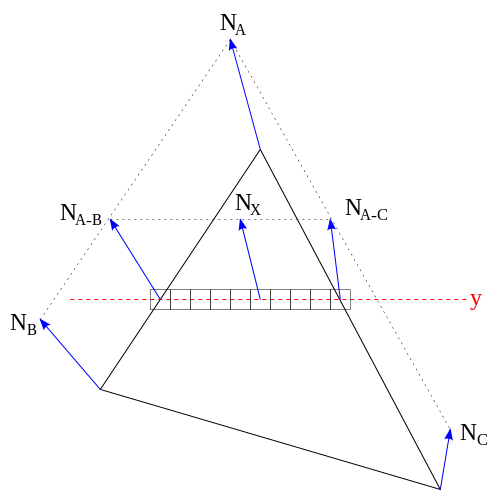
\includegraphics{pics/phongInterpol.png}}
	\caption{Normal interpolation in Phong shading}
	\label{fig:phongInterpo}
\ref{fig:phongInterpo}
\end{figure}

Phong shading works much like Gouraud shading, but rather than interpolating
vertex intensities, the vertex normals are interpolated across the polygon
surface (figure \ref{fig:phongInterpo}), finding a smoothly shifting
normal for each pixel. This normal is then used in the illumination/reflection
model, to find the final intensity weight for that pixel. This will give a more
realistic result that Gouraud shading, at the expense of interpolating normals and
applying the lighting model for each surface pixel. Figure \ref{fig:fVsP}
illustrates the difference in specularity, being quite diffuse in the example
using Gouraud shading, and completely invisible with flat shading.
